% Created 2015-01-20 mar 00:57
\documentclass[xcolor={usenames,svgnames,dvipsnames}]{beamer}
\usepackage[utf8]{inputenc}
\usepackage[T1]{fontenc}
\usepackage{fixltx2e}
\usepackage{graphicx}
\usepackage{longtable}
\usepackage{float}
\usepackage{wrapfig}
\usepackage{rotating}
\usepackage[normalem]{ulem}
\usepackage{amsmath}
\usepackage{textcomp}
\usepackage{marvosym}
\usepackage{wasysym}
\usepackage{amssymb}
\usepackage{hyperref}
\tolerance=1000
\usepackage{color}
\usepackage{listings}
\usepackage{mathpazo}
\usepackage{gensymb}
\usepackage{amsmath}
\bibliographystyle{plain}
\AtBeginSubsection[]{\begin{frame}[plain]\tableofcontents[currentsubsection,sectionstyle=show/shaded,subsectionstyle=show/shaded/hide]\end{frame}}
\AtBeginSection[]{\begin{frame}[plain]\tableofcontents[currentsection,hideallsubsections]\end{frame}}
\usepackage[emulate=units]{siunitx}
\sisetup{per=fraction, fraction=nice, decimalsymbol=comma}
\newunit{\wattpeak}{Wp}
\newunit{\watthour}{Wh}
\newunit{\amperehour}{Ah}
\hypersetup{colorlinks=true, linkcolor=Blue, urlcolor=Blue}
\setbeamercolor{alerted text}{fg=red!50!black} \setbeamerfont{alerted text}{series=\bfseries}
\usetheme[hideothersubsections]{Goettingen}
\usecolortheme{rose}
\usefonttheme{serif}
\author{Oscar Perpiñán Lamigueiro \\ \url{http://oscarperpinan.github.io}}
\date{}
\title{SFCR: Productividad y Sombras}
\hypersetup{
  pdfkeywords={},
  pdfsubject={},
  pdfcreator={Emacs 24.4.1 (Org mode 8.2.7c)}}
\begin{document}

\maketitle

\section{Energía Producida por un SFCR}
\label{sec-1}

\subsection{Procedimiento de cálculo}
\label{sec-1-1}

\begin{frame}[label=sec-1-1-1]{Potencia en un SFCR}
\begin{itemize}
\item Potencia a la Salida del Generador FV
\end{itemize}

$$P_{dc} = A_g \cdot \eta_g(G_{ef}, T_a) \cdot  G_{ef} = %
      \frac{\eta_g(G_{ef}, T_a)}{\eta_g^*} \cdot \frac{G_{ef}}{G^*} \cdot P_g^*$$

\begin{itemize}
\item Potencia a la Salida del Inversor
\end{itemize}

$$P_{ac} = P_{dc} \cdot \eta_{inv}(P_{dc}, V_{dc}) =  P_{dc} \cdot \eta_{inv}(G_{ef}, T_a)$$

\begin{itemize}
\item Energía Producida por un SFCR
\end{itemize}

$$E_{ac} = \int_T \frac{\eta_g(G_{ef}, T_a)}{\eta_g^*} \cdot
      \frac{G_{ef}}{G^*} \cdot \eta_{inv}(G_{ef}, T_a) \cdot P_g^* \mathrm{dt}$$
\end{frame}

\begin{frame}[label=sec-1-1-2]{Energía producida}
$$E_{ac}=P_{g}^{*}\cdot\frac{G_{ef}}{G^*}\cdot PR\cdot (1-FS)$$

\begin{itemize}
\item $E_{ac}$ es la \alert{energía producida} en un periodo.

\item $G^*$ es la \alert{irradiancia} en condiciones estándar de medida (STC,
$G_{stc}=\SI{1}{\kilo\watt\per\meter\squared}$,
$T_c=\SI{25}{\celsius}$)

\item $P_{g}^{*}$ es la \alert{potencia nominal} del generador FV
($\si{\kilo\wattpeak}$) en STC

\item $G_{ef}$ es la \alert{irradiación efectiva incidente} en el plano del
generador

\item $PR$ es el \alert{rendimiento del sistema} o \emph{performance ratio}

\item $FS$ es el \alert{factor de sombras}
\end{itemize}
\end{frame}

\begin{frame}[label=sec-1-1-3]{Productividad}
En algunas ocasiones se habla de \alert{productividad} del sistema, $Y_{f}$,
que es el cociente entre energía producida y potencia nominal del
sistema:
$$Y_{f}=\frac{E_{ac}}{P_{g}^{*}}\,(\si{\kilo\watthour\per\kilo\wattpeak})$$
\end{frame}

\begin{frame}[label=sec-1-1-4]{Performance Ratio}
\begin{itemize}
\item Está concebido para incluir todas las pérdidas que no tienen
dependencia con las condiciones meteorológicas.

\item Este factor \guillemotleft{}puede\guillemotright{} caracterizar el funcionamiento de un sistema
independientemente de la localidad.

\item En sentido estricto no es cierto porque sí hay relación con la
meteorología del lugar.

\item Sin embargo, dado que estos factores son de segundo orden comparados
con la relación entre potencia e irradiancia, suele aceptarse que el
PR sirve para caracterizar la calidad de un sistema fotovoltaico.
\end{itemize}
\end{frame}

\begin{frame}[label=sec-1-1-5]{Performance Ratio}
\begin{block}{Desglose de pérdidas}
\begin{itemize}
\item \alert{Dispersión de parámetros} entre los módulos que componen el
generador (2-4\%)

\item \alert{Tolerancia de potencia} de los módulos respecto a sus
características nominales (3\%)

\item \alert{Temperatura} de funcionamiento de los módulos (5-8\%)

\item Conversión DC/AC realizada por el \alert{inversor} (8-12\%)

\item \alert{Efecto Joule} en los cables (2-3\%)

\item Conversión BT/MT realizada por el \alert{transformador} (2-3\%)

\item \alert{Disponibilidad} del sistema (0,5-1\%)
\end{itemize}
\end{block}
\end{frame}

\begin{frame}[label=sec-1-1-6]{Performance Ratio}
\begin{block}{Valores reales}
\begin{itemize}
\item El análisis de funcionamiento de diversos sistemas FV europeos ha
mostrado que el rango de valores que toma el \emph{performance ratio} es
bastante amplio, con mínimos de 0,4 y máximos de 0,85.

\item Para sistemas instalados desde 1996, \alert{el valor promedio ha sido de
0,74}.
\end{itemize}
\end{block}
\end{frame}

\begin{frame}[label=sec-1-1-7]{Factor de sombras}
\begin{itemize}
\item \alert{El factor de sombras suele tomar valores alrededor del 2 al 4\%},
tanto en instalaciones estáticas como de seguimiento.

\item En casos específicos este factor puede ser más alto (por ejemplo,
debido a la existencia de edificios cercanos, o en aquellas plantas
con un nivel de ocupación de terreno superior al óptimo).
\end{itemize}
\end{frame}

\section{Sombras y ocupación de terreno}
\label{sec-2}

\subsection{Sombras Lejanas}
\label{sec-2-1}

\begin{frame}[label=sec-2-1-1]{Método CTE}
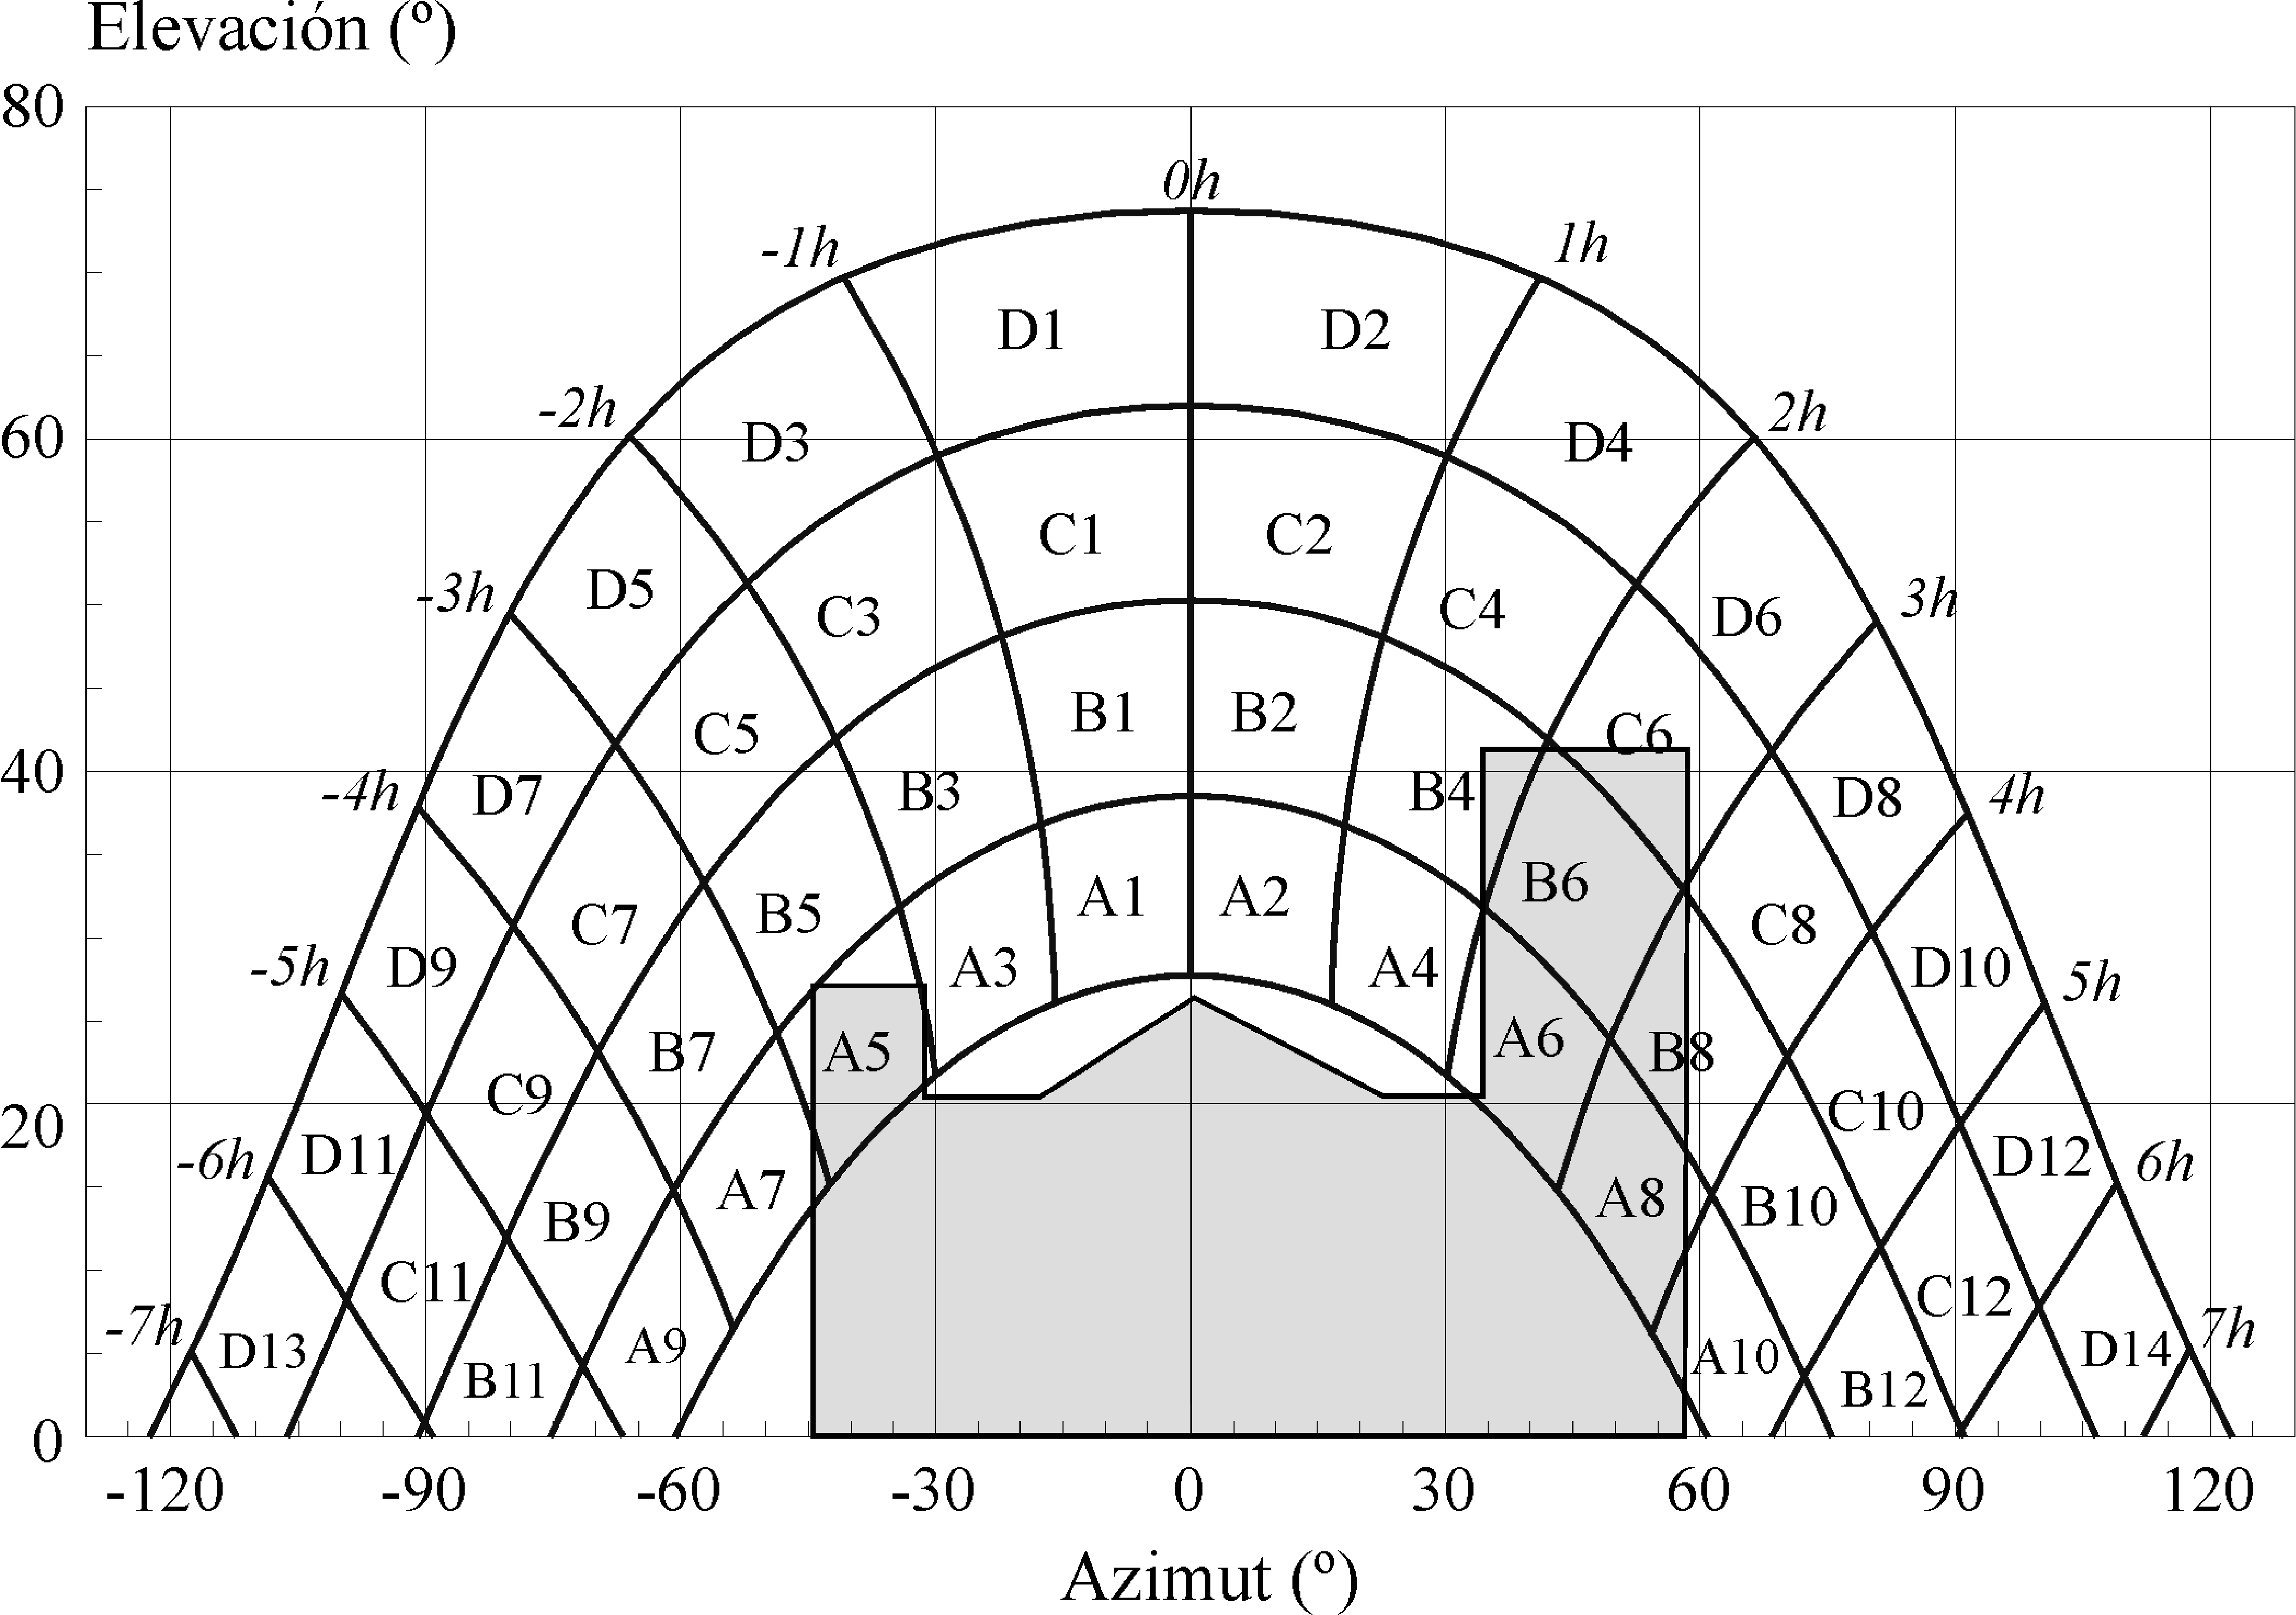
\includegraphics[width=.9\linewidth]{../figs/SombraIES.pdf}
\end{frame}

\subsection{Sombras Cercanas: sistemas estáticos}
\label{sec-2-2}

\begin{frame}[label=sec-2-2-1]{Sombras entre filas}
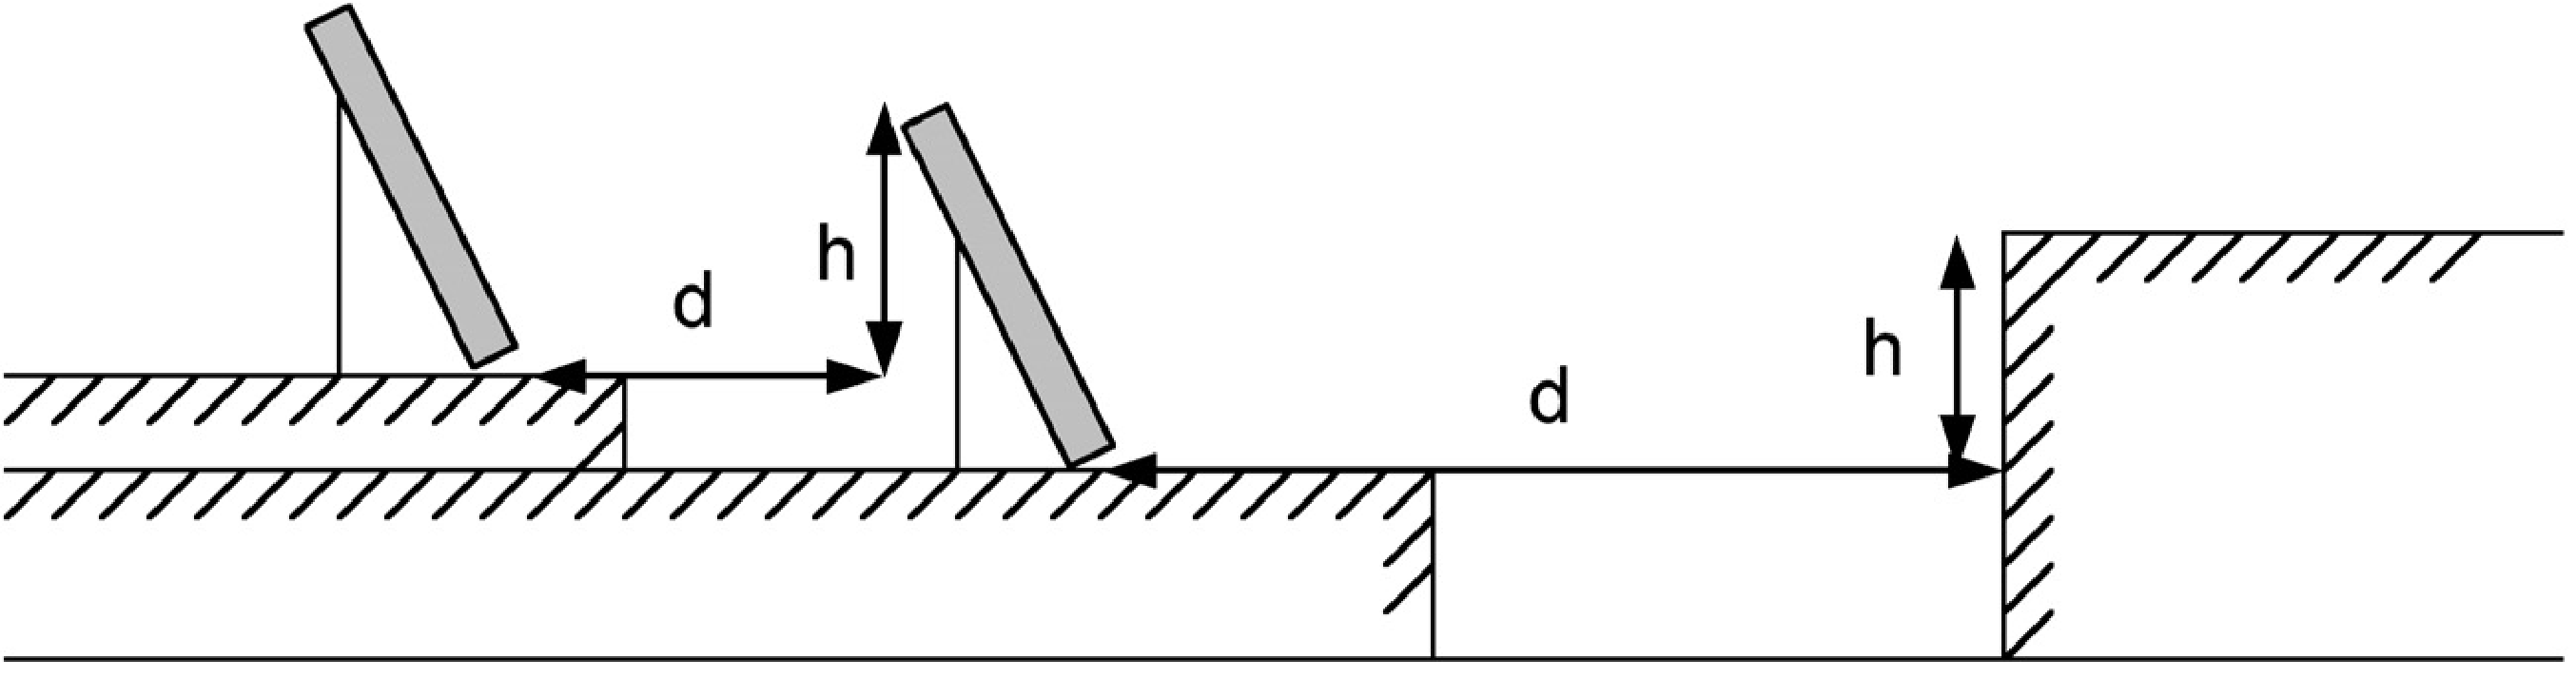
\includegraphics[width=.9\linewidth]{../figs/SombraEstaticaInclinado2.pdf}
\end{frame}

\begin{frame}[label=sec-2-2-2]{Sombras entre filas}
\begin{itemize}
\item Suele establecerse un objetivo de \alert{4 horas de sol en torno al mediodía del solsticio de invierno libres de sombra}.

\item La longitud de la sombra de un obstáculo se mide con:$$d=\frac{h}{\tan\gamma_{s}}$$

\item En el mediodía del solsticio de invierno
\end{itemize}
$$\gamma_{s}=90-23.45-\phi\simeq67-\phi$$ 

\begin{itemize}
\item Para 2 horas antes y después:
\end{itemize}
$$d_{min}=\frac{h}{\tan(61\degree-\phi)}$$
\end{frame}

\subsection{Sombras Cercanas: sistemas de seguimiento}
\label{sec-2-3}

\begin{frame}[label=sec-2-3-1]{Separación de seguidores Doble Eje}
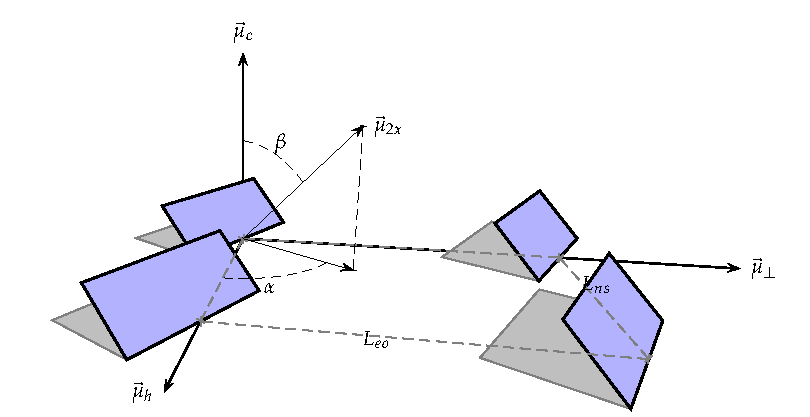
\includegraphics[height=0.5\textheight]{../figs/Sombras2X.pdf}

\begin{columns}
\begin{column}{6cm\textwidth}

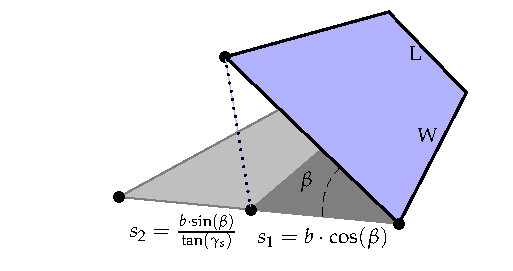
\includegraphics[width=.9\linewidth]{../figs/DimensionesSeguidorSombra.pdf}
\end{column}

\begin{column}{4cm\textwidth}
$$b=\frac{L}{W}$$ 
$$ROT=\frac{L_{ns}\cdot L_{eo}}{b}$$

$$E_{ac}=f(ROT)??$$
\end{column}
\end{columns}
\end{frame}

\begin{frame}[label=sec-2-3-2]{Separación de Seguidores Doble Eje}
$$b=\frac{L}{W}=0.475$$

$$ROT=\frac{L_{ns}\cdot L_{eo}}{b}$$

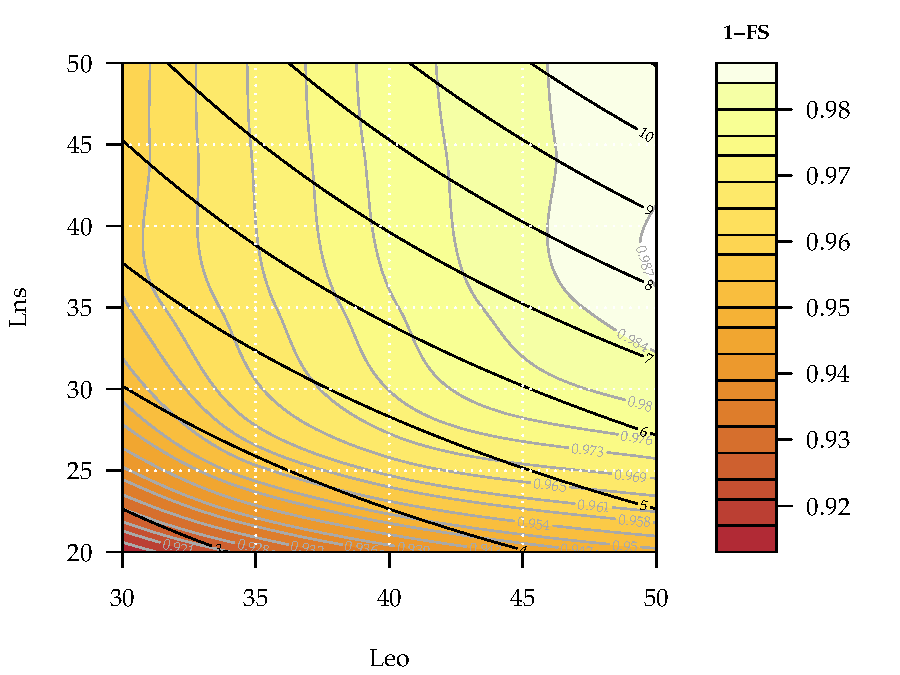
\includegraphics[width=.9\linewidth]{../figs/AbacoSeguidor2X_Ene10.pdf}
\end{frame}


\subsection{Seguidores de eje horizontal NS}
\label{sec-2-4}

\begin{frame}[label=sec-2-4-1]{Separación de Seguidores Eje Horizontal}
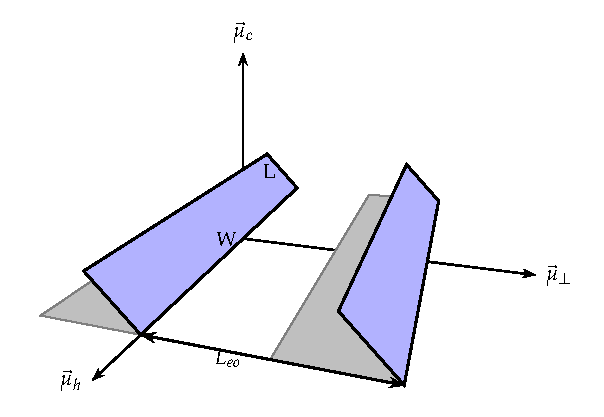
\includegraphics[width=.9\linewidth]{../figs/SombrasHoriz.pdf}

$$W=\infty$$ $$ROT=L_{eo}/L$$
\end{frame}

\begin{frame}[label=sec-2-4-2]{Separación de Seguidores Horizontal N-S}
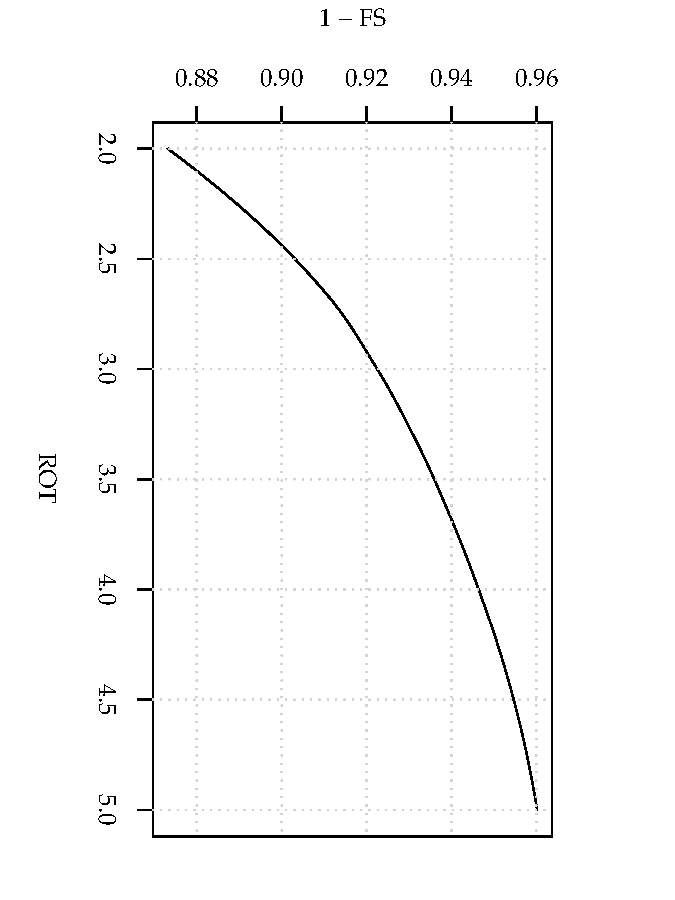
\includegraphics[angle=90,width=.9\linewidth]{../figs/AbacoSeguidorHorizSombra_Ene10.pdf}
\end{frame}

\begin{frame}[label=sec-2-4-3]{Backtracking}
\begin{itemize}
\item El \alert{sombreado} en un generador puede producir problemas por el efecto
de \alert{punto caliente}.

\item En seguidores de eje horizontal se puede \alert{evitar la incidencia de
sombras} en cualquier instante mediante el \guillemotleft{}\alert{backtracking}\guillemotright{}:

\begin{itemize}
\item Al \alert{amanecer} el seguidor está en posición \alert{horizontal}.

\item Según avanza el día el seguidor gira en \alert{sentido contrario al
movimiento solar para evitar las sombras}.

\item En un determinado momento se cruza con el sol y puede continuar el
movimiento \guillemotleft{}convencional\guillemotright{}.

\item En un instante de la tarde debe volver a cambiar el sentido hasta
la \alert{horizontal en la noche}.
\end{itemize}
\end{itemize}
\end{frame}

\begin{frame}[label=sec-2-4-4]{Backtracking}
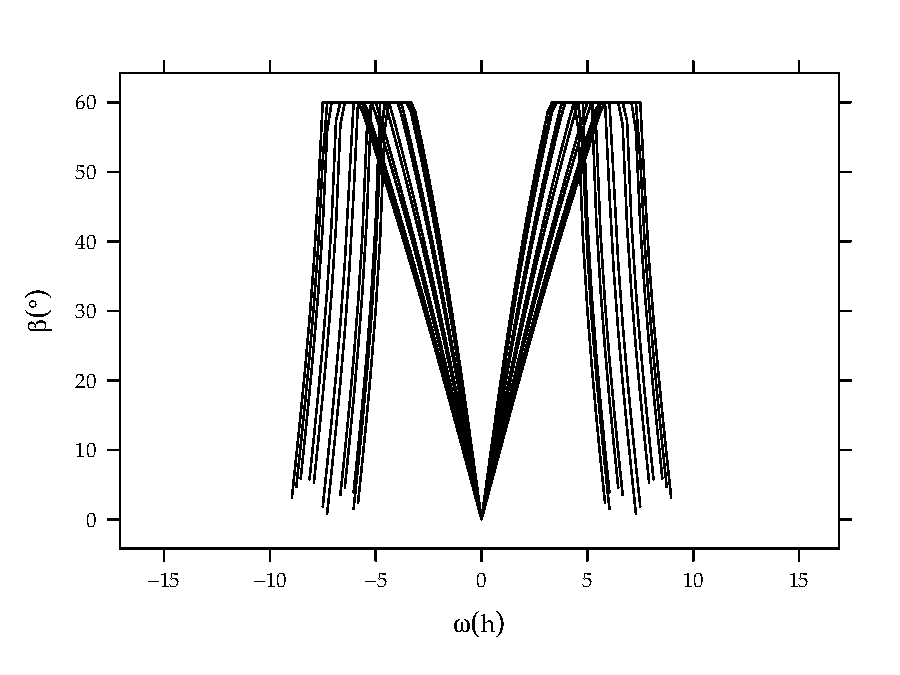
\includegraphics[width=.9\linewidth]{../figs/BackTracking.pdf}
\end{frame}

\begin{frame}[label=sec-2-4-5]{Separación con backtracking}
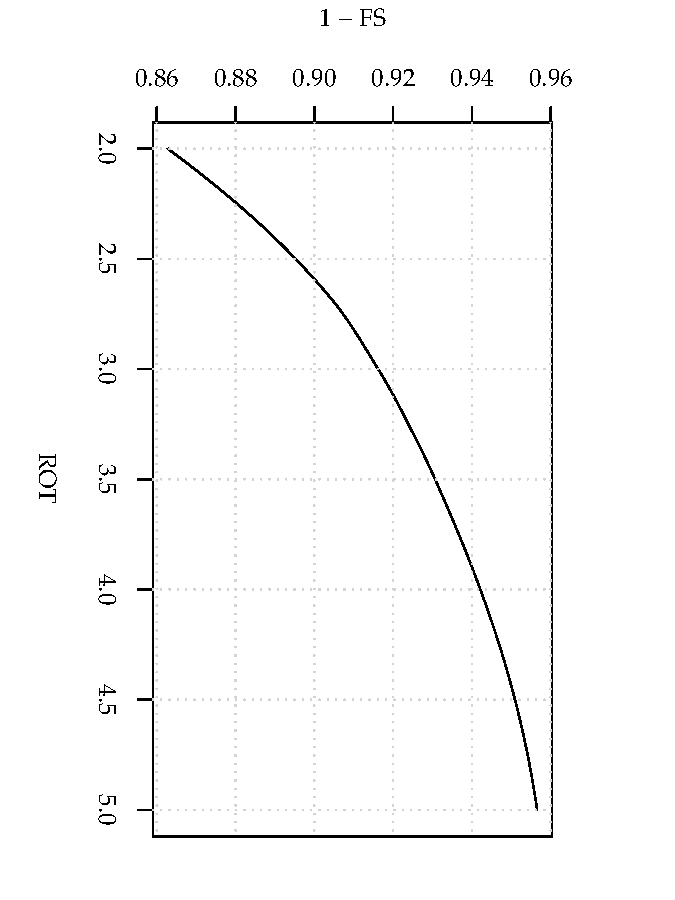
\includegraphics[angle=90,width=.9\linewidth]{../figs/AbacoHorizBT_Ene10.pdf}
\end{frame}

\subsection{Elección de separaciones}
\label{sec-2-5}

\begin{frame}[label=sec-2-5-1]{Elección de separaciones}
La \alert{separación óptima} entre elementos (seguidores o estructuras
estáticas) es aquella que conduce al \alert{mínimo valor del coste de la
energía} producida por el sistema:

\begin{itemize}
\item Con mayor separación disminuyen las \alert{pérdidas por sombreado mutuo},
aumenta la productividad del sistema.

\item Con mayor separación aumentan los \alert{costes relacionados con el area
ocupada} por unidad de potencia.

\item Con mayor separación aumentan los \alert{costes relacionados con los
elementos de unión entre estructuras} (cableado, canalizaciones,
zanjas).
\end{itemize}
\end{frame}

\begin{frame}[label=sec-2-5-2]{Elección de separaciones}
\begin{itemize}
\item Esta separación óptima \alert{depende} de las \alert{estructuras elegidas} y de
las \alert{condiciones económicas} de los elementos.

\item La separación finalmente elegida debe \alert{tomar en consideración las
condiciones del terreno} (fronteras, irregularidades, vaguadas, etc.)
\end{itemize}
\end{frame}

\begin{frame}[label=sec-2-5-3]{Radiación promedio}
$$G_{ef, av} = 1/24 \cdot \left( 10 \cdot G_{ef,0} + 5 \cdot G_{ef,A} + G_{ef,B} + 2 \cdot G_{ef,C} + G_{ef,D} + 5 \cdot G_{ef,E} \right)$$

\begin{columns}
\begin{column}{5cm\textwidth}
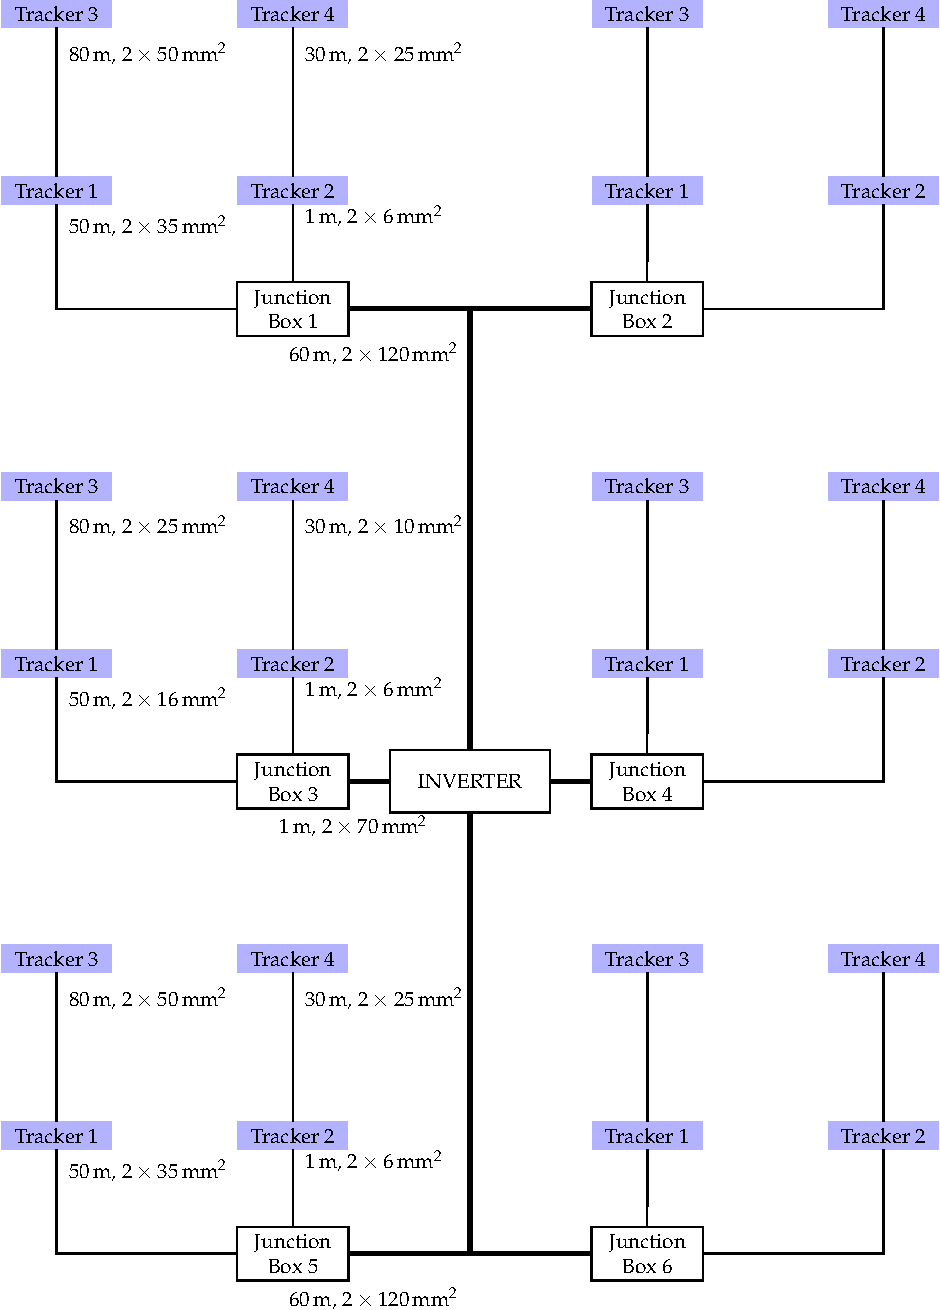
\includegraphics[width=.9\linewidth]{../figs/plantConfiguration.pdf}
\end{column}

\begin{column}{7cm\textwidth}
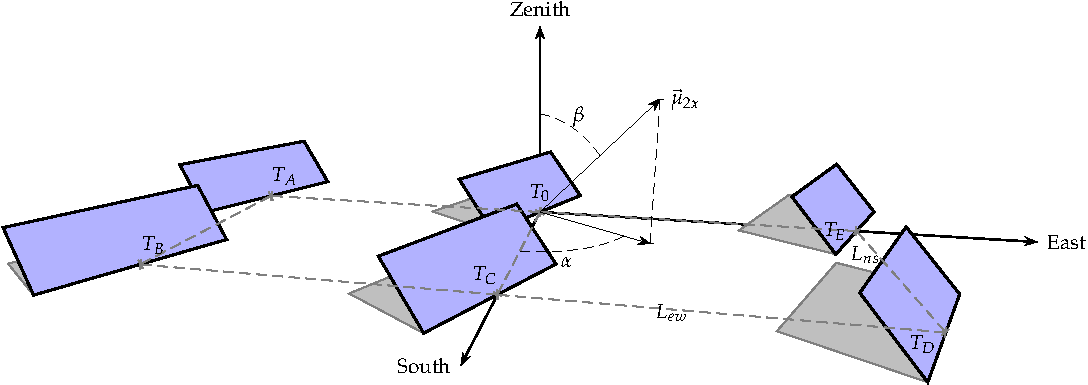
\includegraphics[width=.9\linewidth]{../figs/6trackers.pdf}
\end{column}
\end{columns}
\end{frame}

\begin{frame}[label=sec-2-5-4]{Cableado}
\begin{columns}
\begin{column}{5cm\textwidth}
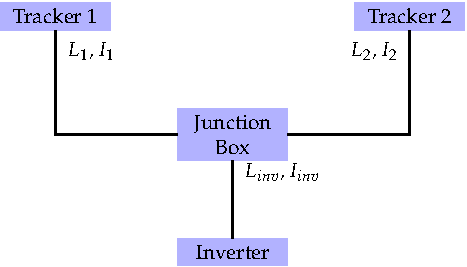
\includegraphics[width=.9\linewidth]{../figs/wiring.pdf}
\end{column}
\begin{column}{6cm\textwidth}
$$\begin{aligned}
    \Delta U_{inv} &= \frac{\Delta U}{1+\sqrt{\frac{\sum_{i=1}^n
          L_{i}^2 \cdot I_{i}}{L_{inv}^2 \cdot I_{inv}}}} \\
    \Delta U_{inv} &+ \Delta U_i = \Delta U\\
    S_{inv} &= 2 \cdot \rho \cdot \frac{L_{inv} \cdot
      I_{inv}}{\Delta U_{inv}} \\
    S_{i} &= 2 \cdot \rho \cdot \frac{L_{i} \cdot I_i}{\Delta U_i}
  \end{aligned}$$
\end{column}
\end{columns}
\end{frame}


\begin{frame}[label=sec-2-5-5]{Coste de la energía producida}
\begin{columns}
\begin{column}{5cm\textwidth}
\begin{itemize}
\item Coste Energía
$$C_E &= \frac{C_P}{E_{AC}}$$
\item Coste Sistema
$$C_p &= C_c + C_A + C_{PV}$$

\item $C_{PV}$ entre $\SI{2.5}{\text{\texteuro}\per\watt}$ y $\SI{5}{\text{\texteuro}\per\watt}$

\item $C_A$ entre $\SI{1.5}{\text{\texteuro}\per\meter\squared}$ y $\SI{4}{\text{\texteuro}\per\meter\squared}$
\end{itemize}
\end{column}

\begin{column}{7cm\textwidth}
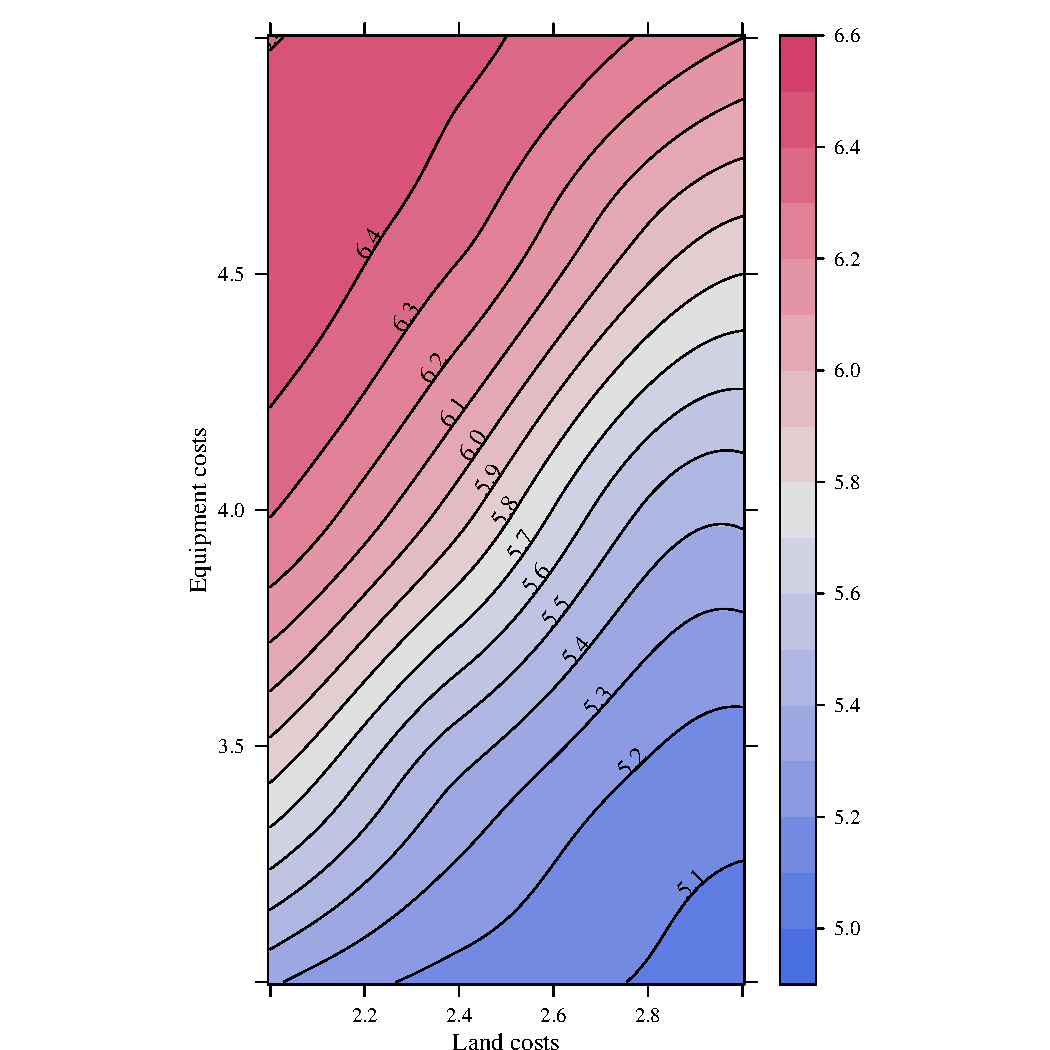
\includegraphics[width=.9\linewidth]{../figs/GRRoptim.pdf}
\end{column}
\end{columns}
\end{frame}

\section{Resumen}
\label{sec-3}

\begin{frame}[label=sec-3-0-1]{Ocupación de terreno y productividad}
\begin{center}
\begin{tabular}{lrl}
SFCR & ROT & Productividad\\
\hline
Estático & 2 & 1\\
Eje Horizontal NS & 4 & 1,05-1,2\\
Doble Eje & 6 & 1,3-1,5\\
\end{tabular}
\end{center}
\end{frame}
% Emacs 24.4.1 (Org mode 8.2.7c)
\end{document}